% Set the document class and theme
\documentclass[notheorems]{beamer}

\setbeamertemplate{theorem}[ams style]
\setbeamertemplate{theorems}[numbered]

\makeatletter
    \ifbeamer@countsect
      \newtheorem{theorem}{\translate{Theorem}}[section]
    \else
      \newtheorem{theorem}{\translate{Theorem}}
    \fi
    \newtheorem{corollary}{\translate{Corollary}}
    \newtheorem{fact}{\translate{Fact}}
    \newtheorem{lemma}{\translate{Lemma}}
    \newtheorem{problem}{\translate{Problem}}
    \newtheorem{solution}{\translate{Solution}}

    \theoremstyle{definition}
    \newtheorem{definition}{\translate{Definition}}
    \newtheorem{definitions}{\translate{Definitions}}

    \theoremstyle{example}
    \newtheorem{example}{\translate{Example}}
    \newtheorem{examples}{\translate{Examples}}

    % Compatibility
    \newenvironment{Lemma}{\begin{lemma}}{\end{lemma}}
    \newenvironment{Proof}{\begin{proof}}{\end{proof}}
    \newenvironment{Theorem}{\begin{theorem}}{\end{theorem}}
    \newenvironment{Problem}{\begin{problem}}{\end{problem}}
    \newenvironment{Corollary}{\begin{corollary}}{\end{corollary}}
    \newenvironment{Example}{\begin{example}}{\end{example}}
    \newenvironment{Examples}{\begin{examples}}{\end{examples}}
    \newenvironment{Definition}{\begin{definition}}{\end{definition}}
\makeatother

\usetheme{Madrid}
\useoutertheme{miniframes} % Alternatively: miniframes, infolines, split
\useinnertheme{circles}

\definecolor{IITHorange}{RGB}{243, 130, 33} % UBC Blue (primary)
\definecolor{IITHyellow}{RGB}{254, 203, 10} % UBC Grey (secondary)

\setbeamercolor{palette primary}{bg=IITHorange,fg=white}
\setbeamercolor{palette secondary}{bg=IITHorange,fg=white}
\setbeamercolor{palette tertiary}{bg=IITHorange,fg=white}
\setbeamercolor{palette quaternary}{bg=IITHorange,fg=white}
\setbeamercolor{structure}{fg=IITHorange} % itemize, enumerate, etc
\setbeamercolor{section in toc}{fg=IITHorange} % TOC sections

% Override palette coloring with secondary
\setbeamercolor{subsection in head/foot}{bg=IITHyellow,fg=white}

\setbeamertemplate{caption}[numbered]
\setbeamertemplate{theorems}[numbered]

\usepackage{./presentation_macros}

\title{The Retracing Boomerang Attack}
\date{April 28, 2025}
\author{Gautam Singh}
\institute[IITH]{Indian Institute of Technology Hyderabad}

\begin{document}
    
    \begin{frame}
        \titlepage
    \end{frame}
    
    \begin{frame}
        \tableofcontents
    \end{frame}
    
    \section{Introduction}
    \label{sec:intro}
    
    \begin{frame}[<+->]{Introduction}
        \begin{enumerate}
            \item Broke the record for 5-round AES when it was
            published.
            \item Brings the attack complexity down to \(2^{16.5}\)
            encryptions.
            \item Uncovers a hidden relationship between boomerang attacks and
            two other cryptanalysis techniques: yoyo game and mixture
            differentials.
        \end{enumerate}
    \end{frame}

    \section{Preliminaries}
    \label{sec:prelims}

    \subsection{Boomerang Attacks}
    \label{subsec:boomerang}

    \begin{frame}{The Boomerang Attack}
        \begin{columns}
            \begin{column}{0.7\textwidth}
                \begin{enumerate}
                    \item<1-> Typically split the encryption function as \(E =
                    E_1 \circ E_0\), with differential trails for each
                    sub-cipher.
                    \item<2-> We can build a distinguisher that can distinguish
                    \(E\) from a truly random permutation in
                    \(\cO\brak{\brak{pq}^{-2}}\) plaintext pairs.
                \end{enumerate}
            \end{column}
            \begin{column}{0.3\textwidth}
                \begin{figure}[!ht]
                    \centering
                    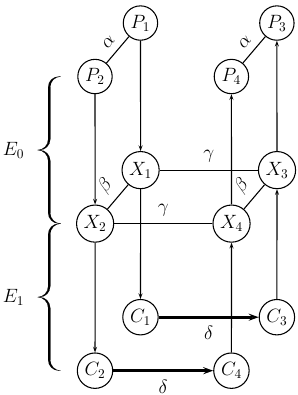
\includegraphics[width=\columnwidth]{images/boomerang.png}
                    \caption{The boomerang attack.}
                    \label{fig:boomerang}
                \end{figure}
            \end{column}
        \end{columns}
    \end{frame}

    \begin{frame}{The Boomerang Distinguisher}
        \vspace{-1em}
        \begin{algorithm}[H]
            \caption{The Boomerang Attack Distinguisher}
            \label{alg:boomerang-dist}
            \begin{algorithmic}[1]
                \State Initialize a counter \(ctr \gets 0\). 
                \State Generate \(\brak{pq}^{-2}\) plaintext pairs \(\brak{P_1, P_2}\)
                such that \(P_1 \oplus P_2 = \alpha\).
                \ForAll {pairs \(\brak{P_1, P_2}\)}
                    \State Ask for the encryption of \(\brak{P_1, P_2}\) to \(\brak{C_1,
                    C_2}\).
                    \State Compute \(C_3 = C_1 \oplus \delta\) and \(C_4 = C_2 \oplus 
                    \delta\). \Comment{\(\delta\)-shift}
                    \State Ask for the decryption of \(\brak{C_3, C_4}\) to \(\brak{P_3,
                    P_4}\).
                    \If {\(P_3 \oplus P_4 = \alpha\)}
                        \State Increment \(ctr\)
                    \EndIf
                \EndFor
                \If {\(ctr > 0\)}
                    \State \Return This is the cipher \(E\)
                \Else
                    \State \Return This is a random permutation
                \EndIf
            \end{algorithmic}
        \end{algorithm}
    \end{frame}

    \subsection{The S-box Switch}
    \label{subsec:s-box-switch}
    
    \begin{frame}[<+->]{Boomerang Switches}
        \begin{enumerate}
            \item Gain 1-2 middle rounds for free by choosing differentials
            carefully. Here, we discuss the \emph{S-box switch}.
            \item Suppose the last operation in \(E_0\) is a layer of S-boxes
            where \(S\brak{\rho_1\|\rho_2\|\ldots\|\rho_t} =
            \brak{f_1\brak{\rho_1}\|f_2\brak{\rho_2}\|\ldots\|f_t\brak{\rho_t}}\)             
            for \(t\) independent keyed functions \(f_i\). Suppose the
            difference for both \(\beta\) and \(\gamma\) corresponding to the
            output of some \(f_j\) is equal to \(\Delta\). 
            \item Denoting this part of the intermediate state by \(X_j\),
            \begin{equation}
                \brak{X_1}_j \oplus \brak{X_2}_j = \brak{X_1}_j \oplus \brak{X_3}_j = \brak{X_2}_j \oplus \brak{X_4}_j = \Delta
                \label{eq:s-switch}
            \end{equation}
            which shows \(\brak{X_1}_j = \brak{X_4}_j\) and \(\brak{X_2}_j =
            \brak{X_3}_j\).
            \item If the differential characteristic in \(f_j^{-1}\) holds for
            \(\brak{X_1, X_2}\), then it will hold for \(\brak{X_3, X_4}\).
            \emph{We pay for probability in one direction}.
            \item Distinguisher probability increases by a factor of
            \(\brak{q^\prime}^{-1}\), where \(q^\prime\) is the probability of
            the differential characteristic in \(f_j\).
        \end{enumerate}
    \end{frame}

    \subsection{The Yoyo Game}
    \label{subsec:yoyo-game}
    
    \begin{frame}[<+->]{The Yoyo Game}
        \begin{enumerate}
            \item Similar to boomerang, starts by encrypting \(\brak{P_1, P_2}\)
            to \(\brak{C_1, C_2}\), then modifying them to \(\brak{C_3, C_4}\)
            and decrypting them.
            \item \emph{Unlike} the boomerang attack, this process continues in
            the yoyo game.
            \item \emph{All} pairs of intermediate values \(\brak{X_{2l + 1},
            X_{2l + 2}}\) satisfy some property (such as zero difference in some
            part).
            \item Probabilities are low with large \(l\). Still, the yoyo
            technique has been used to attack AES reduced to 5 rounds.
        \end{enumerate}
    \end{frame}

    \subsection{Mixture Differentials}
    \label{subsec:mixture}
    
    \begin{frame}{Mixture}
        \begin{definition}[Mixture]
            \label{def:mixture}
            Suppose \(P_i \triangleq \brak{\rho_1^i, \rho_2^i, \ldots,
            \rho_t^i}\). Given a plaintext pair \(\brak{P_1, P_2}\), we say
            \(\brak{P_3, P_4}\) is a \emph{mixture counterpart} of \(\brak{P_1,
            P_2}\) if for each \(1 \le j \le t\), the quartet \(\brak{\rho_j^1,
            \rho_j^2, \rho_j^3, \rho_j^4}\) consists of two pairs of equal
            values or of four equal values. The quartet \(\brak{P_1, P_2, P_3,
            P_4}\) is called a \emph{mixture}.
        \end{definition}
        \pause
        \begin{enumerate}
            \item<2->  If \(\brak{P_1, P_2, P_3, P_4}\) is a mixture, then XOR
            of the intermediate values \(\brak{X_1, X_2, X_3, X_4}\) is zero.
            \item<3-> \(X_1 \oplus X_3 = \gamma \implies X_2 \oplus X_4 =
            \gamma\). Hence, for \(\gamma \xrightarrow{q} \delta\) in \(E_1\),
            \(C_1 \oplus C_3 = C_2 \oplus C_4 = \delta\) with probability
            \(q^2\).
            \item<4-> Has been applied to AES reduced up to 6 rounds. \(E_0\) is
            taken to be the first 1.5 rounds of AES, which can be treated as
            four parallel super S-boxes.
        \end{enumerate}
    \end{frame}

    \section{The Retracing Boomerang Attack}
    \label{sec:retr-boomerang}
    
    \subsection{The Retracing Boomerang Framework}
    \label{sec:retr-framework}

    \begin{frame}{The Retracing Boomerang Framework}
        \begin{figure}[!ht]
            \centering
            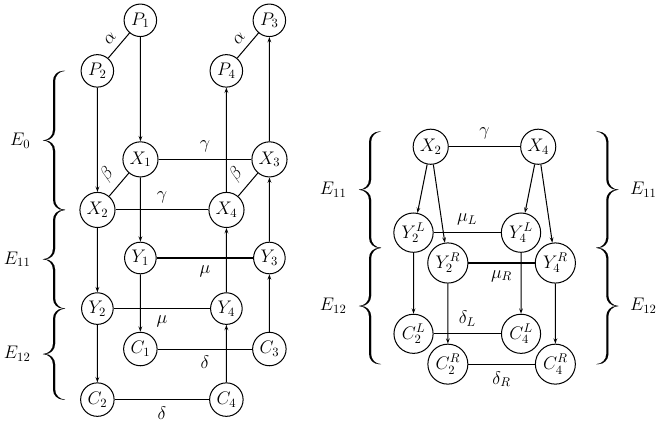
\includegraphics[width=0.6\columnwidth]{images/retracing_boomerang.png}
            \caption{The retracing boomerang attack.}
            \label{fig:retr-boomerang}
        \end{figure}
    \end{frame}

    \begin{frame}[<+->]{The Retracing Boomerang Attack}
        \begin{enumerate}
            \item The \emph{retracing boomerang} framework consists of a
            \emph{shifting} type and a \emph{mixing} type.
            \item Both attacks use the setup shown in \cref{fig:retr-boomerang}.
            \item Although the additional split looks restrictive, it applies
            for a wide class of block ciphers such as SASAS constructions.
            \item Further, we assume that \(E_{12}\) can be split into two parts
            of size \(b\) and \(n - b\) bits, call these functions \(E_{12}^L\)
            and \(E_{12}^R\), with characteristic probabilities \(q_2^L\) and
            \(q_2^R\) respectively.
        \end{enumerate}
    \end{frame}

    \subsection{The Shifting Retracing Attack}
    \label{subsec:shift-retr-boomerang}

    \begin{frame}[<+->]{The Shifting Retracing Boomerang Attack}
        \begin{enumerate}
            \item Adds a \(\brak{b - 1}\)-bit filtering in the middle of the
            attack procedure.
            \item Check if \(C_1^L \oplus C_2^L = 0 \textrm{ or } \delta_L\).
            \emph{Discard all such pairs that do not satisfy this relation}.
            \item A \(\delta\)-shift is performed on the filtered ciphertext
            pairs to get \(\brak{C_3, C_4}\).
            \item Filtering ensures that the two unordered pairs \(\brak{C_1,
            C_3}\) and \(\brak{C_2, C_4}\) are \emph{equal}.
            \item If one of these pairs satisfies the differential
            characteristic \(\delta_L \xrightarrow{q_2^L} \mu_L\), \emph{the
            other pair will too!}.
            \item Increases the probability of the boomerang distinguisher by
            \(\brak{q_2^L}^{-1}\).
            \item Any possible characteristic of \(\brak{E_{12}^L}\) has
            probability at least \(2^{-b + 1}\), thus the overall probability
            increases by a factor of at most \(2^{b - 1}\). On the other hand,
            filtering only leaves \(2^{-b + 1}\) of the pairs, so there is no
            apparent gain.
        \end{enumerate}
    \end{frame}

    \begin{frame}{The Shifting Retracing Boomerang Attack}
        \begin{figure}
            \centering
            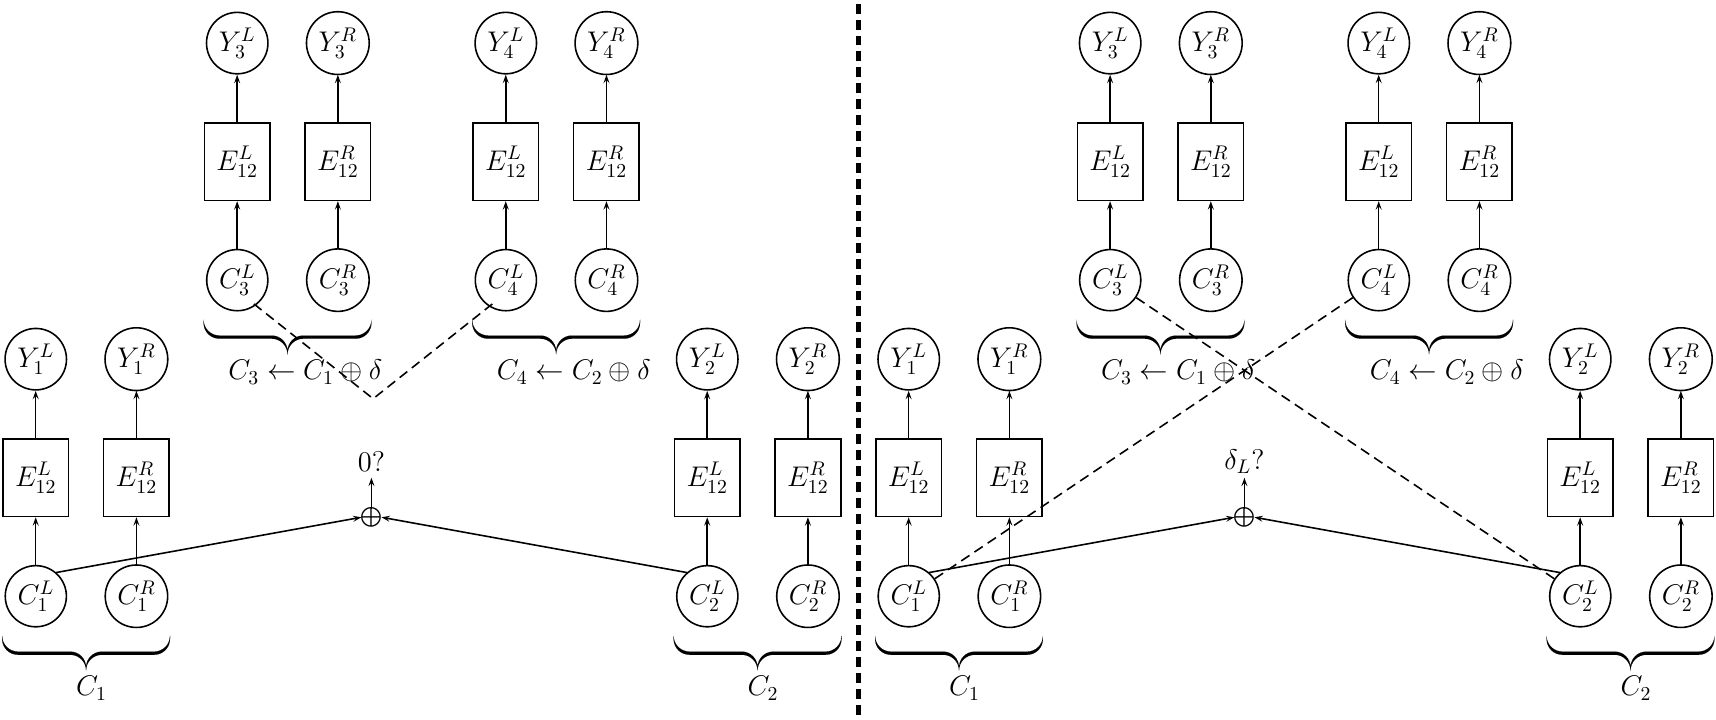
\includegraphics[width=\columnwidth]{images/shifting_boomerang.png}
            \caption{A shifted quartet (dashed lines indicate equality).}
        \end{figure}
    \end{frame}

    \begin{frame}[<+->]{Advantages of Filtering}
        \begin{enumerate}
            \item \emph{Improving the signal to noise ratio.} Improving the
            probability by a factor of \(\brak{q_2^L}^{-1}\) improves the SNR
            which ensures a higher fraction of the filtered pairs on average
            satisfy \(P_3 \oplus P_4 = \alpha\). The characteristic \(\beta
            \xrightarrow{p} \alpha\) in the backward direction for the pair
            \(\brak{X_3, X_4}\) can be replaced by a truncated differential
            characteristic \(\beta \xrightarrow{p^\prime} \alpha^\prime\) of
            higher probability.
            \item \emph{Reducing the data complexity.} Due to the filtering, the
            attack leaves fewer ciphertexts. This improves the complexity in
            cases where more decryption queries are made.
            \item \emph{Reducing the time complexity.} The filtering can also
            reduce the time complexity if it is dominated by the analysis of the
            plaintext pairs \(\brak{P_3, P_4}\).
        \end{enumerate}
    \end{frame}

    \subsection{The Mixing Retracing Attack}
    \label{subsec:mix-retr-boomerang}

    \begin{frame}[<+->]{The Mixing Retracing Boomerang Attack}
        \begin{enumerate}
            \item In the shifting attack, the attacker forces equality between
            the unordered pairs \(\brak{C_1^L, C_2^L}\) and \(\brak{C_3^L,
            C_4^L}\) using a \(\delta\)-shift.
            \item In this type of attack, each ciphertext pair can be shifted by
            \(\brak{C_1^L \oplus C_2^L, 0}\). The resulting ciphertexts are
            \begin{align}
                C_3 &= \brak{C_3^L, C_3^R} = \brak{C_1^L \oplus \brak{C_1^L \oplus C_2^L}, C_1^R} = \brak{C_2^L, C_1^R}, \\
                C_4 &= \brak{C_4^L, C_4^R} = \brak{C_2^L \oplus \brak{C_1^L \oplus C_2^L}, C_2^R} = \brak{C_1^L, C_2^R}.
            \end{align}
            \item Again, the unordered pairs \(\brak{C_1^L, C_2^L}\) and
            \(\brak{C_3^L, C_4^L}\) are equal.
            \item Further, \(C_1^R = C_3^R\) and \(C_2^R = C_4^R\), thus we gain
            an \emph{additional} factor of \(\brak{q_2^R}^{-2}\) for a total
            probability of \(\brak{pq_1}^2q_2^L\), \emph{better than shifting}!
            \item Similar to the core step used in the yoyo attack on AES.
        \end{enumerate}
    \end{frame}

    \begin{frame}{The Mixing Retracing Boomerang Attack}
        \begin{figure}
            \centering
            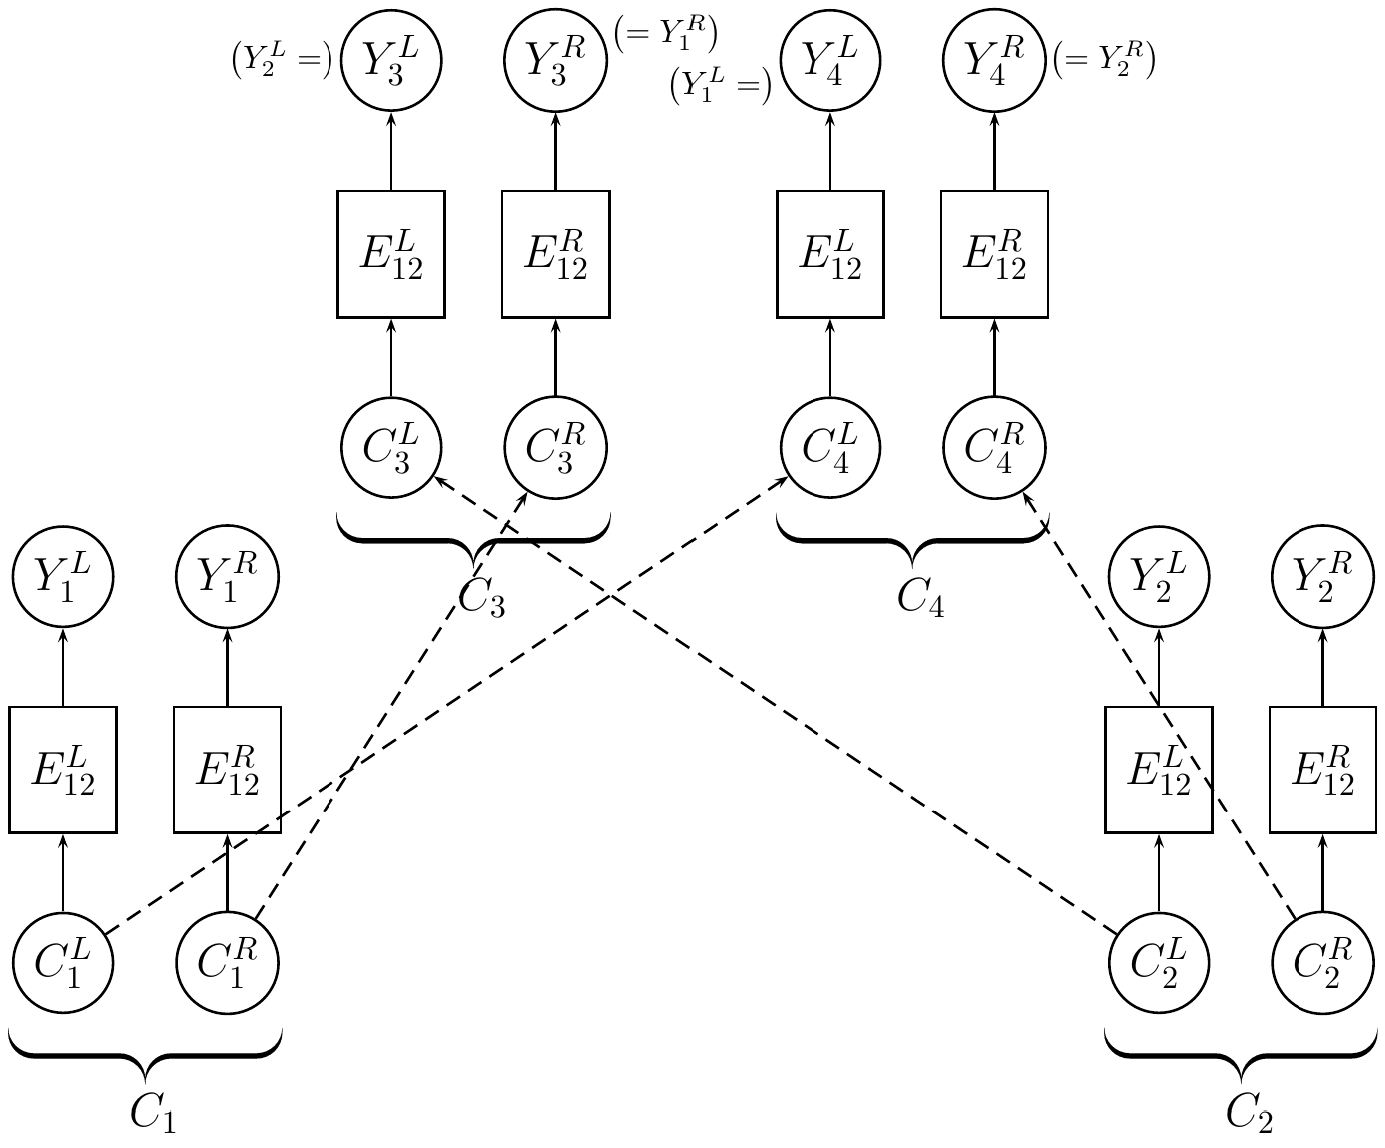
\includegraphics[width=0.55\columnwidth]{images/mixing_boomerang.png}
            \caption{A mixture quartet of ciphertexts (dashed lines indicate equality).}
        \end{figure}
    \end{frame}

    \subsection{Comparison Between the Two Types of Retracing Attacks}
    \label{subsec:cmp}
    \begin{frame}[<+->]{Advantages of Shifting Retracing Attack}
        \begin{enumerate}
            \item \textbf{Using structures}
            \begin{itemize}[<+->]
                \item Shifting applies the same \(\delta\)-shift to all pairs of
                ciphertexts.
                \item Filtering is applied first to reduce the data complexity.
                \item Not possible in mixing: shift is based on ciphertexts, no
                filtering.
                \item Basic boomerang attacks add a round at the top or bottom
                of the distinguisher. With shifting, one can obtain all
                ciphertexts, shift them by \(\delta\) and then decrypt,
                simulatneously checking for the filter and condition between
                \(P_3\) and \(P_4\) using a hash table.
            \end{itemize}
            \item \textbf{Combination with \(E_{11}\)}
            \begin{itemize}[<+->]
                \item In mixing, the output difference of \(E_{12}^L\) is
                arbitrary.
                \item Usually no good combination between characteristics of
                \(\brak{E_{12}^L}^{-1}\) and \(\brak{E_{11}}^{-1}\). For
                instance, in the yoyo attack, \(E_{11}\) is empty.
            \end{itemize}
            \item \textbf{Construction of `friend pairs'}
            \begin{itemize}[<+->]
                \item `Friend pairs' are pairs which satisfy a common property.
                \item More `friend pairs' can be constructed in the shifting
                variant.
            \end{itemize}
        \end{enumerate}
    \end{frame}

    \section{Retracing Boomerang Attack on Five Round AES}
    \label{sec:retr-boomerang-aes}

    \subsection{Brief Description of AES}
    \label{subsec:aes-description}
    \begin{frame}{Description of AES, Notation}
        \begin{enumerate}[<+->]
            \item Byte ordering shown after \(SB\) in \cref{fig:aes} (column
            major).
            \item \(j\)-th byte of a state \(X_i\) is denoted as \(X_{i,j}\) or
            \(\brak{X_i}_j\).
            \item Denote by \(W, Z\) and \(X\) the states before \(MC\) in round
            0, at the input to round 1 and before \(MC\) in round 2
            respectively.
            \item The \(l\)-th shifted column (resp. \(l\)-th inverse shifted
            column) refers to application of \(SR\) (resp. \(SR^{-1}\)) to the
            \(l\)-th column.
            \item Round subkeys are \(k_{-1}, k_0, \ldots\).
        \end{enumerate}
        \begin{figure}[!ht]
            \centering
            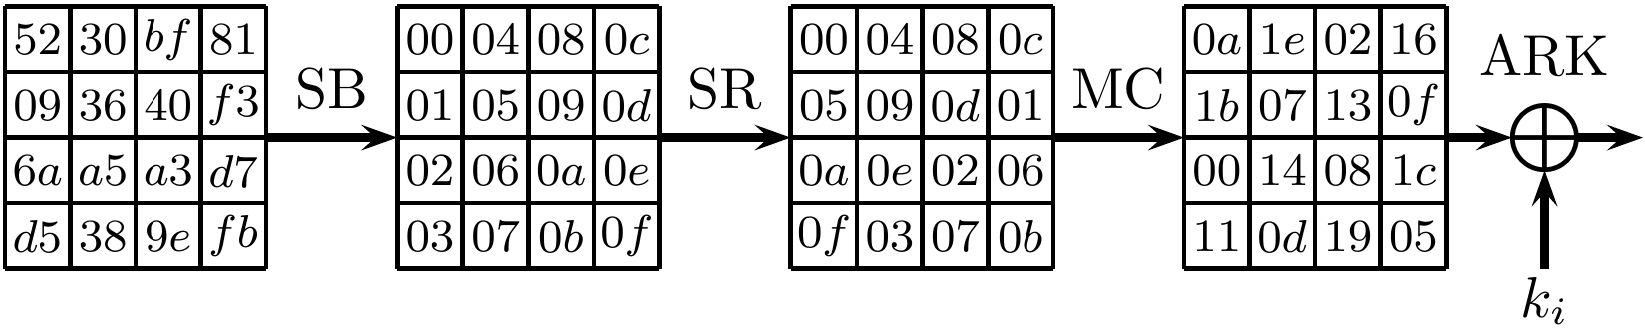
\includegraphics[width=0.9 \columnwidth]{images/aes.png}
            \caption{An AES round.}
            \label{fig:aes}
        \end{figure}
    \end{frame}

    \subsection{The Yoyo Attack on Five Round AES}
    \label{subsec:yoyo-aes}

    \begin{frame}[<+->]{Summary of Yoyo Attack on Five Round AES}
        \begin{enumerate}
            \item Decomposes AES as \(E = E_{12} \circ E_{11} \circ E_0\) where
            \(E_0\) is the first 2.5 rounds, \(E_{11}\) is the MC of round 2 and
            \(E_{12}\) is the last 2 rounds.
            \item Truncated differential characteristic for \(E_0\): zero input
            difference in three inverse shifted columns and zero output
            difference in a single shifted column with probability \(4 \cdot
            2^{-8} = 2^{-6}\). (\emph{why?})
            \item For \(E_{12}\), 1.5 rounds of AES can be taken as four 32-bit
            super S-boxes.
            \item Ciphertext pair \(\brak{C_1, C_2}\) modified into its mixture
            \(\brak{C_3, C_4}\) w.r.t. super S-boxes and decrypted. The four
            inputs to the S-boxes have zero XOR, thus \(X_1 \oplus X_2 \oplus
            X_3 \oplus X_4 = 0\) since MC is linear. 
            \item \(X_3 \oplus X_4 = 0\) in a shifted column and \(Z_3 \oplus
            Z_4 = 0\) in an inverse shifted column with probability \(2^{-6}\).
            This corresponds to one of the four quartets \(\brak{0,5,10,15}\),
            \(\brak{1,4,11,14}\), \(\brak{2,5,8,13}\), \(\brak{3,6,9,12}\).
            \item Attack quartets of \(k_{-1}\). Friend pairs of \(\brak{Z_3,
            Z_4}\) used to get more information.
        \end{enumerate}
    \end{frame}

    \begin{frame}{Algortihm of Yoyo Attack}
        \begin{algorithm}[H]
            \caption{Yoyo Attack on Five Round AES}
            \label{alg:yoyo-aes}
            \algrenewcommand\alglinenumber[1]{\scriptsize ####1:}
            \scriptsize
            \begin{algorithmic}[1]
                \State Ask for the encryption of \(2^6\) pairs \(\brak{P_1,
                P_2}\) of chosen plaintexts with non-zero difference only in 
                bytes \(0, 5, 10, 15\).
                \For {all corresponding ciphertext pairs \(\brak{C_1, C_2}\)}
                    \State Let \(\brak{C_3^j, C_4^j}\), \(j = 1, 2, 3, 4\) be
                    the mixture counterparts of the pair \(\brak{C_1, C_2}\).
                    \State Ask for the decryption of the ciphertext pairs and
                    consider the pairs \(\brak{Z_3^j, Z_4^j}\).
                    \ForAll {\(l \in \cbrak{0, 1, 2, 3}\)}
                        \State Assume all four pairs \(\brak{Z_3^j, Z_4^j}\) and
                        the pair \(\brak{Z_1, Z_2}\) have zero difference in 
                        byte \(l\).
                        \State Use the assumption to extract bytes \(0, 5, 10,
                        15\) of \(k_{-1}\).
                        \If {a contradiction is reached}
                            \State Increment \(l\)
                            \If {\(l > 3\)}
                                Discard the pair
                            \EndIf
                        \Else
                            \State Using \(Z_3^j \oplus Z_4^j = 0\) in the
                            entire \(l\)-th inverse shifted column, attack the
                            three remaining columns of round 0 (sequentially)
                            and decude the rest of \(k_{-1}\).
                        \EndIf
                    \EndFor
                \EndFor
            \end{algorithmic}
        \end{algorithm}
    \end{frame}

    \begin{frame}{Meet in the Middle Improvement on Yoyo Attack}
        
    \end{frame}

The yoyo attack has data complexity about \(2^9\) and overall time complexity is
\(2^{40}\). A careful analysis of round 0 can reduce the complexity down to
\(2^{31}\) encryptions. However, there is a better improvement that can be made
using a meet in the middle (MITM) attack on bytes 0, 5, 10 and 15 of \(k_{-1}\).
Denote the intermediate value of byte \(m\) before the \(MC\) operation of round
0 during encryption as \(W_m\), and consider WLOG \(l = 0\). Then, the input to
round 1 satisfies
\begin{equation}
    Z_0 = 02_x \cdot W_0 \oplus 03_x \cdot W_1 \oplus 01_x \cdot W_2 \oplus 01_x \cdot W_3.
    \label{eq:mitm}
\end{equation} 
In the MITM attack, the adversary guesses bytes 0, 5 of \(k_{-1}\) by computing
the values
\begin{equation}
    02_x \cdot \brak{\brak{W_3^j}_0 \oplus \brak{W_4^j}_0} \oplus 03_x \cdot \brak{\brak{W_3^j}_1 \oplus \brak{W_4^j}_1}
    \label{eq:mitm-0-5}
\end{equation}
for \(j = 1, 2, 3\), concatenating these values and storing them in a table for
each guess. Similarly, the adversary guesses the values for bytes 10, 15 of
\(k_{-1}\) and computes 
\begin{equation}
    01_x \cdot \brak{\brak{W_3^j}_2 \oplus \brak{W_4^j}_2} \oplus 01_x \cdot \brak{\brak{W_3^j}_3 \oplus \brak{W_4^j}_3}
    \label{eq:mitm-10-15}
\end{equation}
for \(j = 1, 2, 3\) and checks for a match in the table, which is equivalent to
the condition \(\brak{Z_3^j}_0 = \brak{Z_4^j}_0\) for \(j = 1, 2, 3\). This
24-bit filtering leaves \(2^8\) candidates for bytes 0, 5, 10, 15 of \(k_{-1}\).
These can be checked by using the conditions \(\brak{Z_3^4}_0 = \brak{Z_4^4}_0\)
and \(\brak{Z_1}_0 = \brak{Z_2}_0\).

Although the data complexity looks like \(2^{16}\), the \emph{dissection
technique} can be used to maintain the memory at \(2^9\). The time complexity is
now reduced to \(2^6 \cdot 4 \cdot 2^{16} = 2^{24}\) operations, which is
roughly equivalent to less than \(2^{23}\) encryptions.

\end{document}
